\documentclass[12pt]{article}
\usepackage{graphicx}
\usepackage[margin=2cm, a4paper]{geometry}
\usepackage{setspace}
\usepackage{pdfpages}
\usepackage{float}
\usepackage{amsmath}
\usepackage{fancyvrb}
\usepackage{amssymb}
\usepackage{minted}
\usepackage{enumitem}
\usepackage[colorlinks,linkcolor=blue]{hyperref}


\renewcommand{\contentsname}{Contents}
\renewcommand{\figurename}{Figure}
\renewcommand{\tablename}{Table}
\hypersetup{
    colorlinks=true,
    linkcolor=black,
    filecolor=magenta,      
    urlcolor=blue,
}
\newcommand{\mytitle}{CSIE 2344, Spring 2026: Laboratory 1}
\newcommand{\myauthor}{B13902022 Richard Lai}

\usepackage{fancyhdr}
\pagestyle{fancy}
\fancyhead{}
\fancyhead[L]{\mytitle}
\fancyhead[R]{\myauthor}


\title{\mytitle}
\author{\myauthor}
\date{\today}

\begin{document}
\maketitle

\section{Source Code}
\subsection{}
\begin{minted}[frame=lines,framesep=2mm,baselinestretch=1.2,linenos,breaklines]{verilog}
module rca_gl(
	output C3,       // carry output
	output[2:0] S,   // sum
	input[2:0] A, B, // operands
	input C0         // carry input
	);

	wire c1, c2;
	FA fa0(c1, S[0], A[0], B[0], C0);
	FA fa1(c2, S[1], A[1], B[1], c1);
	FA fa2(C3, S[2], A[2], B[2], c2);
	
endmodule
\end{minted}

\subsection{}
\begin{minted}[frame=lines,framesep=2mm,baselinestretch=1.2,linenos,breaklines]{verilog}
module cla_gl(
    output C3,       // carry output
    output[2:0] S,   // sum
    input[2:0] A, B, // operands
    input C0         // carry input
    );

    wire [2:0] g, p, p_xor;
    wire c1, c2;

    AND g_and0(g[0], A[0], B[0]);
    AND g_and1(g[1], A[1], B[1]);
    AND g_and2(g[2], A[2], B[2]);

    OR p_or0(p[0], A[0], B[0]);
    OR p_or1(p[1], A[1], B[1]);
    OR p_or2(p[2], A[2], B[2]);

    XOR p_xor0(p_xor[0], A[0], B[0]);
    XOR p_xor1(p_xor[1], A[1], B[1]);
    XOR p_xor2(p_xor[2], A[2], B[2]);

    wire p0c0;
    AND and_p0c0(p0c0, p[0], C0);
    OR or_c1(c1, g[0], p0c0);

    wire g0p1, c0p0p1, c2_tmp;
    AND and_c0p0p1(c0p0p1, p[1], p0c0);
    AND and_g0p1(g0p1, g[0], p[1]);
    OR or_c2tmp(c2_tmp, g[1], g0p1);
    OR or_c2(c2, c2_tmp, c0p0p1);

    wire g1p2, g0p1p2, c0p0p1p2;
    AND4 and4_c0p0p1p2(c0p0p1p2, C0, p[0], p[1], p[2]);
    AND and_g0p1p2(g0p1p2, g0p1, p[2]);
    AND and_g1p2(g1p2, g[1], p[2]);

    OR4 or4_c3(C3, g[2], g1p2, g0p1p2, c0p0p1p2);

    XOR xor_s0(S[0], p_xor[0], C0);
    XOR xor_s1(S[1], p_xor[1], c1);
    XOR xor_s2(S[2], p_xor[2], c2);
endmodule
\end{minted}

\section{Waveform}
\begin{figure}[H]
    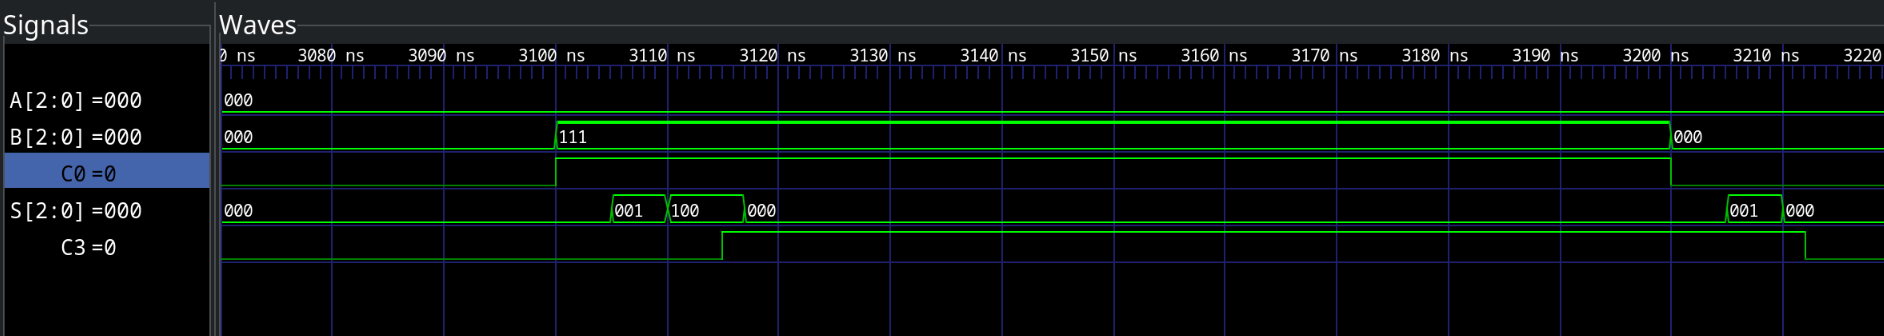
\includegraphics[width=\linewidth]{cla_wave1.png}
\end{figure}
\section{Propagation Delays}
\subsection{}
The maximum delay is 23 ticks on transition 000+000+0 $\rightarrow$ 000+111+1.
\subsection{}
The maximum delay is 17 ticks on transition 000+000+1 $\rightarrow$ 000+000+0.

\end{document}
% how to display codes?
% \begin{minted}[frame=lines,framesep=2mm,baselinestretch=1.2,linenos,breaklines]{python}
% \end{minted}

% how to display images?
% \begin{figure}[H]
%     \centering
%     \includegraphics[width=0.5\linewidth]{}
%     \caption{Caption}
% \end{figure}
% test
